\documentclass{beamer}
\input{../utils/preamble}
\createdgmtitle{11}
%--------------------------------------------------------------------------------
\begin{document}
%--------------------------------------------------------------------------------
\begin{frame}[noframenumbering,plain]
\titlepage
	\resetonslide
\end{frame}
%=======
\begin{frame}{Recap of Previous Lecture}
	\myfootnotewithlink{https://arxiv.org/abs/2011.13456}{Song Y., et al. Score-Based Generative Modeling through Stochastic Differential Equations, 2020}
	\vspace{-0.3cm}
	\[
		d\bx = \bff(\bx, t) dt + g(t) d \bw \qquad \text{(SDE with the probability path $p_t(\bx)$)}
	\]
	\vspace{-0.7cm}
	\begin{block}{Probability Flow ODE}
		There exists an ODE with the identical probability path $p_t(\bx)$ of the form:
		\vspace{-0.3cm}
		\[
			d\bx = \bv(\bx, t) dt, \quad \bv(\bx, t) = \bff(\bx, t) -\frac{1}{2} g^2(t) \frac{\partial}{\partial \bx} \log p_t(\bx)
		\]
		\vspace{-0.7cm}
	\end{block}
	\begin{figure}
		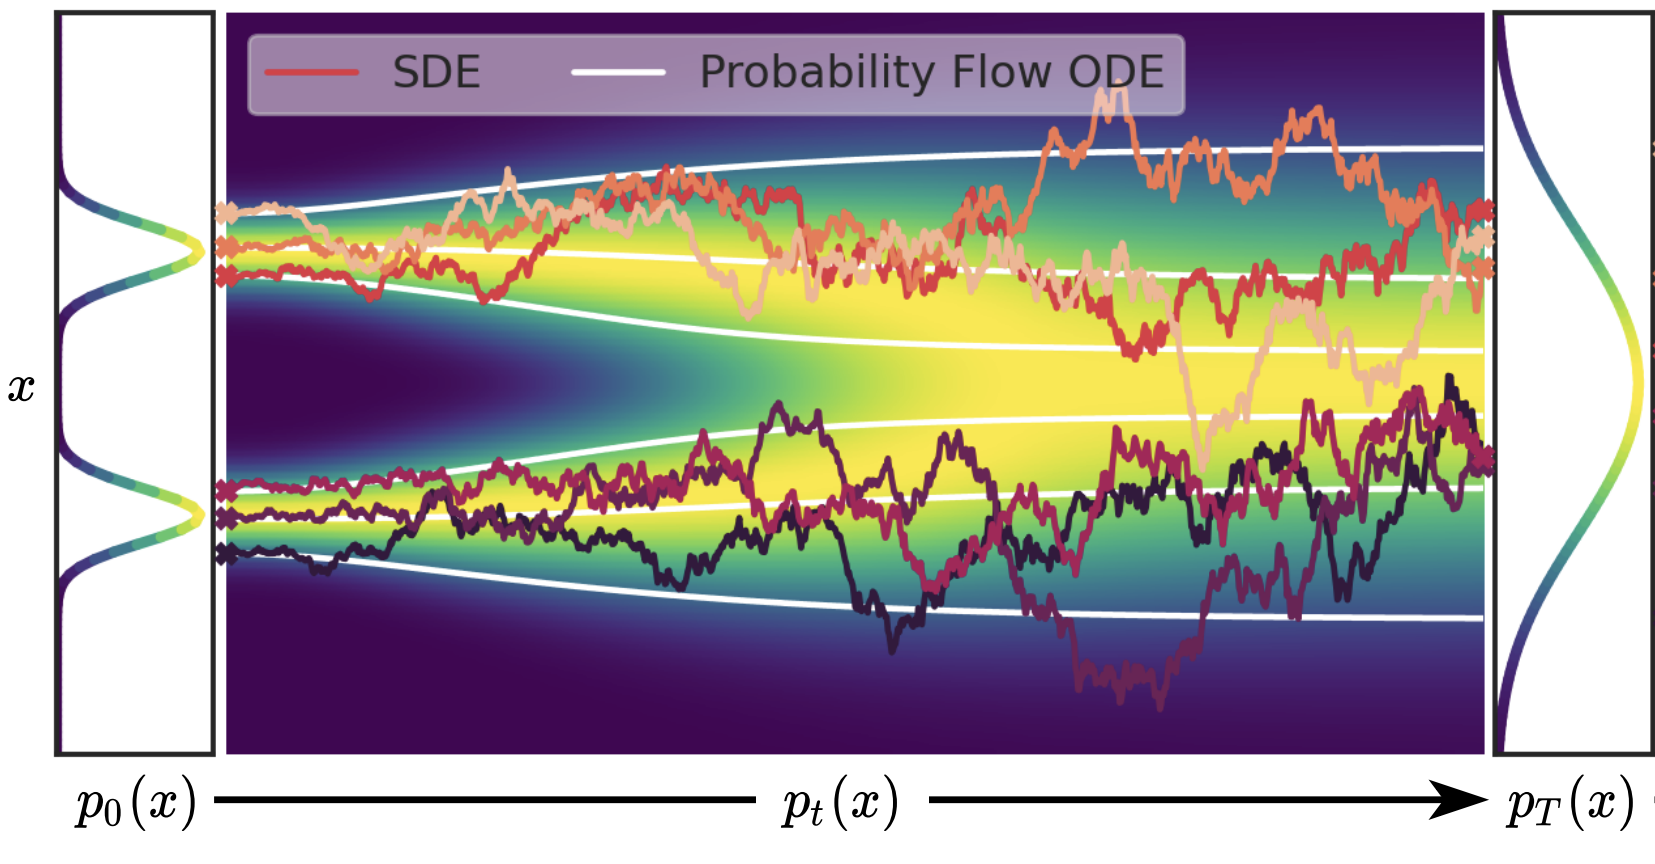
\includegraphics[width=0.75\linewidth]{figs/probability_flow}
	\end{figure}
\end{frame}
%=======
\begin{frame}{Outline}
	\tableofcontents
\end{frame}
%=======
\section{Conditional Flow Matching}
%=======
\begin{frame}{Generative Models Taxonomy}
	\renderTaxonomy{fm}
\end{frame}
%=======
\begin{frame}{Flow Matching}
    \myfootnotewithlink{https://arxiv.org/abs/2302.00482}{Tong A., et al. Improving and Generalizing Flow-Based Generative Models with Minibatch Optimal Transport, 2023}
	Let's introduce the latent variable $\bz$:
	\[
		p_t(\bx) = \int p_t(\bx | \bz) p(\bz) d \bz 
	\]
	Here, $p_t(\bx | \bz)$ is a \textbf{conditional probability path}.
	\eqpause
	The conditional probability path $p_t(\bx | \bz)$ satisfies the KFP theorem:
	\[
		\frac{\partial p_t(\bx | \bz)}{\partial t} = - \diver\left(\bv(\bx, \bz, t) p_t(\bx | \bz)\right),
	\]
	where $\bv(\bx, \bz, t)$ is a \textbf{conditional vector field}:
	\eqpause
	\[
		\frac{d\bx_t}{dt} = \bv(\bx_t, t) \quad \Rightarrow \quad \frac{d\bx_t}{dt} = \bv(\bx_t, \bz, t)
	\]
	\vspace{-0.3cm}
\end{frame}
%=======
\begin{frame}{Flow Matching}
    \myfootnotewithlink{https://arxiv.org/abs/2302.00482}{Tong A., et al. Improving and Generalizing Flow-Based Generative Models with Minibatch Optimal Transport, 2023}
	\begin{block}{Flow Matching (FM)}
		\vspace{-0.3cm}
		\[
			\bbE_{t \sim U[0, 1]} \bbE_{\bx \sim p_t(\bx)}\left\| \bv(\bx, t) - \bv_{\btheta}(\bx, t) \right\|^2 \rightarrow \min_{\btheta}
		\]
		\vspace{-0.3cm}
	\end{block}
	\begin{block}{Conditional Flow Matching (CFM)}
		\vspace{-0.3cm}
		\[
			\bbE_{t \sim U[0, 1]} \bbE_{\bz \sim p(\bz)} \bbE_{\bx \sim p_t(\bx | \bz)}\left\| \bv(\bx, \bz, t) - \bv_{\btheta}(\bx, t) \right\|^2 \rightarrow \min_{\btheta}
		\]
		\vspace{-0.5cm}
	\end{block}
    \eqpause
	\begin{block}{Theorem}
		If $\supp(p_t(\bx)) = \bbR^m$, then the optimal value of the FM objective equals the optimal value of the CFM objective.
	\end{block}
    \eqpause
	\begin{block}{Proof}
		This can be proved in a similar way as in the denoising score matching theorem.
	\end{block}
\end{frame}
%=======
\begin{frame}{Conditional Flow Matching}
    \myfootnotewithlink{https://arxiv.org/abs/2302.00482}{Tong A., et al. Improving and Generalizing Flow-Based Generative Models with Minibatch Optimal Transport, 2023}
	\begin{block}{Theorem}
		\vspace{-0.7cm}
		\begin{multline*}
			\argmin_{\btheta} \bbE_{t \sim U[0, 1]} \bbE_{\bx \sim p_t(\bx)}\left\| \bv(\bx, t) - \bv_{\btheta}(\bx, t) \right\|^2 = \\
			= \argmin_{\btheta} \bbE_{t \sim U[0, 1]} \bbE_{\bz \sim p(\bz)} \bbE_{\bx \sim p_t(\bx | \bz)}\left\| \bv(\bx, \bz, t) - \bv_{\btheta}(\bx, t) \right\|^2
		\end{multline*}
		\vspace{-0.7cm}
	\end{block}
    \eqpause
	\begin{block}{Proof}
		\vspace{-0.5cm}
		{\small
		\begin{multline*}
			\bbE_{\bx \sim p_t(\bx)}\left\| \bv(\bx, t) - \bv_{\btheta}(\bx, t) \right\|^2 = \\ 
			= {\color{olive}\bbE_{\bz \sim p(\bz)} \bbE_{\bx \sim p_t(\bx | \bz)}}\left[\| \bv_{\btheta}(\bx, t) \|^2 - 2 {\color{teal}\bv_{\btheta}^\top(\bx, t)\bv(\bx, t)} \right] + \text{const}(\btheta)
		\end{multline*}
		}
		\eqpause
		\vspace{-1.0cm}
		{\small
		\begin{multline*}
			\bbE_{p_t(\bx)} \left[{\color{teal}\bv_{\btheta}^\top(\bx, t)\bv(\bx, t)} \right] = \int p_t(\bx) \left[\bv_{\btheta}^\top(\bx, t) \left( \int p_t(\bz | \bx)\bv(\bx, \bz, t)d\bz \right) \right] d\bx 
			\nextonslide{ = \\ = \int \int {\color{violet}p_t(\bx) p_t(\bz | \bx)} \left[\bv_{\btheta}^\top(\bx, t) \bv(\bx, \bz, t) \right] d\bz d\bx}
			\nextonslide{ = \\ = {\color{violet}\bbE_{p(\bz)} \bbE_{p_t(\bx | \bz)}} \left[\bv_{\btheta}^\top(\bx, t) \bv(\bx, \bz, t) \right]}
		\end{multline*}
		}
	\end{block}
\end{frame}
%=======
\begin{frame}{Conditional Flow Matching: Training and Sampling}
	\myfootnotewithlink{https://arxiv.org/abs/2210.02747}{Lipman Y., et al. Flow Matching for Generative Modeling, 2022}
	\[
		\bbE_{t \sim U[0, 1]} \bbE_{\bz \sim p(\bz)} \bbE_{\bx \sim p_t(\bx | \bz)}\left\| \bv(\bx, \bz, t) - \bv_{\btheta}(\bx, t) \right\|^2 \rightarrow \min_{\btheta}
	\]
	\[
		\bbE_{p(\bz)} p_0(\bx | \bz) = \cN(0, \bI); \quad \bbE_{p(\bz)} p_1(\bx | \bz) = \pd(\bx).
	\]
	\eqpause
	\vspace{-0.3cm}
	\begin{block}{Training}
		\begin{enumerate}
			\item Sample a time $t \sim U[0, 1]$ and $\bz \sim p(\bz)$.
			\item Draw $\bx_t \sim p_t(\bx | \bz)$.
			\item Compute the loss $ \cL = \left\| \bv(\bx_t, \bz, t) - \bv_{\btheta}(\bx_t, t) \right\|^2 $.
		\end{enumerate}
	\end{block}
	\eqpause
	\begin{block}{Sampling}
		\begin{enumerate}
			\item Sample $\bx_0 \sim \cN(0, \bI)$.
			\item Solve the ODE to obtain $\bx_1$:
			\[
				\bx_1 = \bpsi_1(\bx_0) = \ODESolve_v(\bx_0, \btheta, t_0=0, t_1=1).
			\]
		\end{enumerate}
	\end{block}
\end{frame}
%=======
\begin{frame}{Summary}
	\begin{itemize}	
		\item Conditional flow matching introduces the latent variable $\bz$, reformulating the initial task in terms of conditional dynamics.
	\end{itemize}
\end{frame}
%=======
\end{document}